% 
%jff-notes
%
\documentclass[11pt]{article}
\usepackage[pdftex]{graphicx}
\usepackage{amssymb}
\usepackage{latexsym}
%\usepackage{relsize}
\usepackage{textcomp}
%processed for 10 pt 
%\documentstyle[epsf,psfig]{article}
%\documentstyle[epsf]{article}
\oddsidemargin 0pt
\topmargin -0.0cm
\textwidth 6.2in
\textheight 8.5in
\baselineskip 18pt
%\renewcommand{\baselinestretch} {1.5}
\newenvironment{nitemize}
   {\begin{list}{\begin{math}\bullet\end{math}}%
      {\setlength{\leftmargin}{5mm}
       \setlength{\topsep}{1mm}
       \setlength{\parsep}{0in}
       \setlength{\itemsep}{.7mm}}}%
   {\end{list}}

\newcommand{\fract}[2]{\frac{\textstyle #1}{\textstyle #2}}
\newcommand{\trans}[3]{#1 \stackrel{#2}{\longrightarrow} #3}
\newcommand{\notrans}[3]{#1 \stackrel{#2}{\not\! \longrightarrow} #3}
\bibliographystyle{plain}
\begin{document}
\title{A simple RTTY plugin for SDRuno}
\author{
Jan van Katwijk\\
Lazy Chair Computing \\
The Netherlands\\
{\em J.vanKatwijk@gmail.com}}
%\date{}
\maketitle
%\baselineskip 22pt
\ \\
\ \\
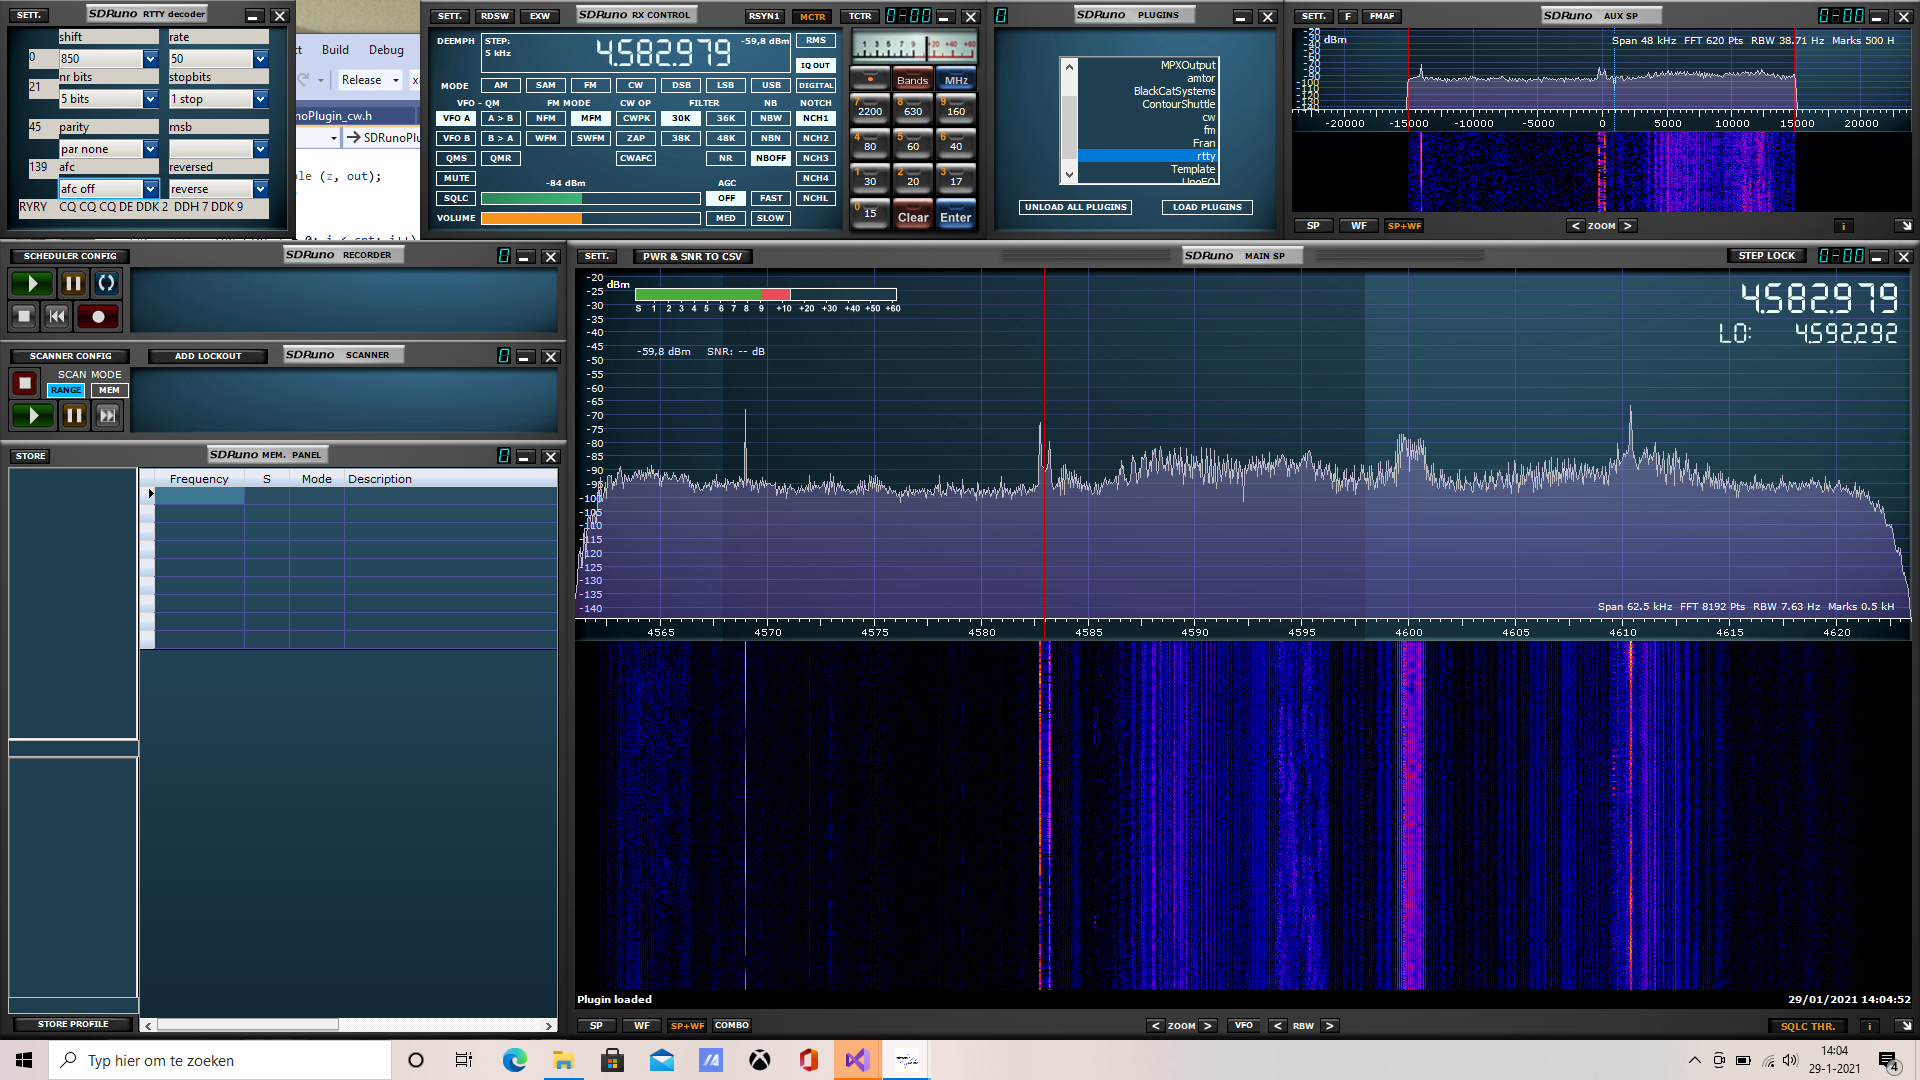
\includegraphics[width=140mm]{rtty-example.png}
\ \\
\section{Introduction}
The SDRuno rtty plugin is a simple plugin to decode rtty signals.

There are still some service transmissions on shortwave, one that
I often use when testing is on 4583 KHz, and of course
there are from time to time plenty amateur transmissions around 14085 KHz,
The main difference between commercial and service transmissions and the
amateur transmissions are the signal width and the duration.
\par
As is well known, an rtty signal is FSK modulated, during transmission
of a letter or digit,  mark and space signals are transmitted alternately.
Mark and space differ 170 Hz in frequency
for amateur transmissions and 850 to 1000 Hz for commecial and
service transmissions.

\section{Settings}
For amateur modes, rrty is a signal with a small footprint, the distance
betwene the mark and the space signal is 170 Hz, 
The decoder therefore works with a low intermediate samplerate, 
12000 samples/second. Since the minimal samplerate for the
SDRplay family is 2000000, a lot of decimation has to be done.
\par
This implementation requires an input sample rate of 62500 samples/second,
this requires the setting of the mainwidget to a samplerate of 2000000,
and a decimation of 32, as shown in the picture
One should realize that the SDRuno spectrum display shows a band of 62.5
KHz, the advantage is that one sees a lot of signals, the disadvantage
is that precise tuning, based on the view on the spectrum is not easy.

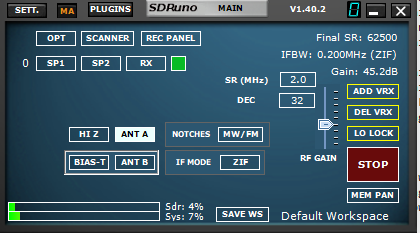
\includegraphics[width=100mm]{main-widget.png}

The plugin generates an audiotone of 800 Hz + the tuning offset, in my
experience is sound very helpful in precise tuning.

The sound is output with a rate of 48000, setting "AM" in the RX control window
will set this rate.

\section{Tuning}
As e.g. psk, rtty for amateur bands, is a signal with a small footprint,
and since many of the amateur transmissions are brief messages
(such as CQ CQ ...), tuning requires some training.
\par
What is really helpful here  is the auxiliary spectrum display, the widget
can be enlarged, and one can zoom into getting a
view on a app 1 KHz spectrum.

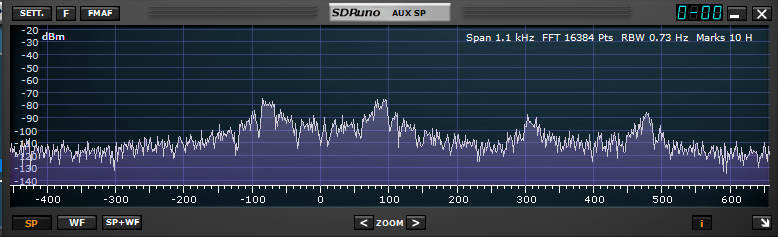
\includegraphics[width=100mm]{auxiliary-spectrum-display.png}

The way to tune is in two steps
\begin{itemize}
\item coarse tuning with the mouse on the main spectrum display;
\item fine tuning with the mouse controlled numerical display until the
mark and space signals  are left resp. right of the '0' in the auxiliary spectrum display.
\end{itemize}

\section{The plugin}
The plugin widget  is shown in the picture

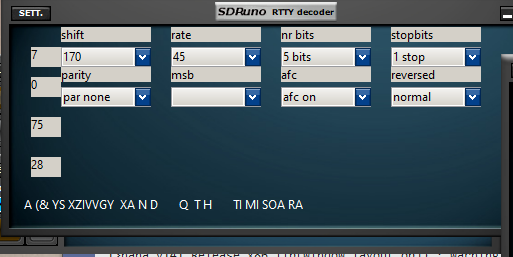
\includegraphics[width=100mm]{rtty-plugin-widget.png}

The widget has eight control comoboxes and there are 4 small numeric
labels.

The picture shows that the received message is slightly garbled at the start
but then, synchdonization was obtained and the qth could be deciphered.

The controls are, from left to right and from top to bottom
\begin{itemize}
\item The shift, rtty supports a number of shifts, i.e. distances
between mark and space signal;
\item the baudrate, rtty supports a  umber of different baudrate,
for the amateur bands the rate is 45;
\item the number of bits. The normal setting is 5 bits per letter, with
\item stopbits, with one stop bit.
\item Usually there are no parity bits,
\item the bit order (i.e. is the first bit the msb or the lsb bit) is
normal.
\item not related to the decoding is the setting of the afc, as shown in the
picture, the afc is on . The result is depicted in the top two number
displays on the left. The top one indicates the accumulated offset
for the frequency correction, the second indicates the error detected
after applying the offset. Here it shows that the frequency was 7 Hz off, and
after correcting the frequency, there was no residual error.
\item the combobox with label {\em reversed} allows switching the
mark and the space signals.
\end{itemize}

Finally, the two number labels at the left, these can be ignored, the
top of the two denotes an attempt to estimate the baudrate (since the
actual baudrate is 45, the estimate of 75 is off), the bottom one
displays the measured average offset of the mark and the space signal
relative to the center frequency.
\end{document}


